
\section{System design}
A generic \ac{UOWC} system incorporates a source generating information to be
transmitted, a transmission modulator onto the optical carrier, a transmitter
equipped with projection optics and beam steering elements to focus and steer
the beam, a detector converting optical to electrical signals and then a
subsequent signal processing unit and demodulator.

\subsection{Transmitter}
The transmitter normally uses the blue-green portion of the spectrum.
Output power can range from 10 mW to 10 W. Lasers or \ac{LED}s can be used.
Lasers have faster switching time (meaning higher data rates can be supported
as the modulation bandwidth higher) and higher optical power (meaning higher
range), but \ac{LED}s are cheaper, simpler, less temperature dependent and
more reliable. Lasers have a much smaller viewing angle than \ac{LED}s.

\subsection{Receiver}
The receiver should have a wide \ac{FOV}, high gain and provide high \ac{SNR}.
They are photo sensors that come in a range of types.

According to the literature, currently semiconductor photo-sensors (mainly
\ac{PIN} photodiodes) are the best fit for \ac{UOWC}.

\subsubsection{\ac{APD}}
A highly sensitive semiconductor that exploits the photoelectric effect to
convert light to electricity.

*** This is from first-sensor.com *** \\
As in the case of standard diodes, photons generate electron-hole pairs,
which are accelerated by the applied external voltage such that further
electrons are introduced to the conduction band by means of impact ionization.
These secondary electrons can in turn absorb sufficient energy to raise further
electrons into the conduction band. A multiplication factor of several hundred
can thus be achieved.

Avalanche diodes are usually employed in the case of very low optical signal
strengths, but are also used for applications with high modulation frequencies.
As of frequencies of approx. 60 MHz, the noise level heightened by the
avalanche effect is generally lower than that produced by a conventional diode
in combination with external electronic amplification.

\subsubsection{\ac{SPAD}}
*** This is from Wikipedia ***\\
A solid-state photodetector in which a photon-generated carrier (via the
internal photoelectric effect) can trigger a short-duration but relatively
large avalanche current.

The fundamental difference between SPADs and APDs is that SPADs are
specifically designed to operate with a reverse-bias voltage well above the
breakdown voltage. This kind of operation is also called Geiger-mode in the
literature (as opposed to the linear-mode for the case of an APD).

\subsubsection{\ac{PMT}}
A vacuum tube which is very sensitive to light. They have high gain, low noise,
a high frequency response and a large collection area, but they are also large,
have higher power consumption and are quite fragile.

\subsection{Modulation Schemes}
There are two types of modulation schemes that can be used for \ac{UOWC}.
The laser can either be directly modulated, also known as Intensity Modulation
or a carrier can be introduced after the laser which the signal can be
modulated on to, known as Coherent Modulation.

\subsubsection{Intensity Modulation}
This is the most widely used modulation scheme, where the intensity of the
optical carrier is modulated using the source data directly. Either the
message signal or an external modulator can be used. They are low cost and
less complex.

Techniques for modulation include \ac{OOK}, \ac{PPM} and phase shifting
techniques. \ac{PPM} has better power efficiency and is thus better for
battery operated devices.

\subsubsection{Coherent Modulation}
This uses a local oscillator to down convert the optical carrier to baseband
or to \ac{RF} intermediate frequency (which is then subsequently demodulated
to baseband). The \ac{SNR} can be improved due to the use of the local
oscillator. These systems are more complex and higher cost, and use more power
than intensity modulated systems.

Phase coherent modulation schemes give better \ac{BER} performance than
intensity modulation schemes.

Coherent modulation schemes can be implemented by using an electro-optic
modulator.

\begin{figure}[H]
  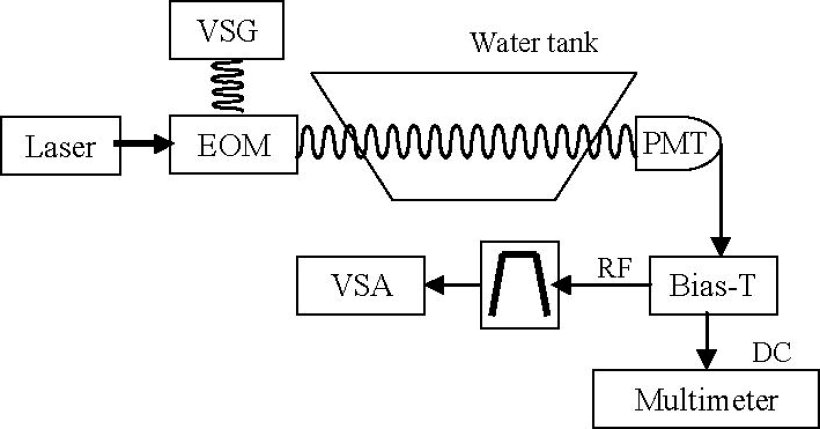
\includegraphics[width=0.8\textwidth]{coherent-source.jpg}
  \caption{Coherent Modulation using electro-optic modulator
	   \cite{cochenour_mullen_laux_2007}}
  \label{fig:boat1}
\end{figure}

\subsection{Channel Coding Schemes}
Error coding schemes can help mitigate the effect of underwater attenuation.
Redundant bits are introduced into the transmitted bit sequence so that the
receiver can correct a limited number of errors in the received message.
This is known as \ac{FEC}.

It would be best to use convolutional codes if possible, as they can provide
much higher \ac{BER} performance under harsh environments.

\subsubsection{Block Codes}
These codes add extra bits to each block, known as parity bits. These carry
no extra information. They are simple to implement but are not as good as
convolutional codes especially in turbid water or multiple scatters. Examples
are \ac{RS} codes.

\subsubsection{Convolutional Codes}
Each code word depends on the message block but also a number of previous
message blocks. This requires sequential logic circuits to implement and is
thus harder to implement. They do however provide much higher performance.
Examples are \ac{LDPC} and Turbo codes.
